\documentclass[a4paper,oneside,14pt]{extreport}

\usepackage[T2A]{fontenc}
\usepackage[utf8]{inputenc}
\usepackage[english,russian]{babel}

\usepackage[left=30mm, right=10mm, top=20mm, bottom=20mm, bindingoffset=0cm]{geometry}

\usepackage{microtype}
\usepackage{tikz}

\usepackage{setspace}
\onehalfspacing
\usepackage{graphicx}
\usepackage{indentfirst}
\setlength{\parindent}{12.5mm}

\usepackage{titlesec}
\titleformat{\chapter}{\LARGE\bfseries}{\thechapter}{10pt}{\LARGE\bfseries}
\titlespacing*{\chapter}{0pt}{-20pt}{10pt}
\titleformat{\section}{\large\bfseries}{\thesection}{10pt}{\large\bfseries}
\titlespacing*{\section}{0pt}{0pt}{10pt}
\titleformat{\subsection}{\normalsize\bfseries}{\thesubsection}{10pt}{\normalsize\bfseries}
\titlespacing*{\subsection}{0pt}{5pt}{5pt}

\addto{\caption}{\renewcommand*{\contentsname}{Содержание}}
\usepackage[square,sort,comma,numbers]{natbib}
\renewcommand{\bibsection}{\chapter*{Список литературы}}

\usepackage{caption}

\usepackage{wrapfig}
\usepackage{float}
\usepackage{listings}
\usepackage{graphicx}
\graphicspath{{.}}
\newcommand{\imgwc}[4]
{
	\begin{figure}[#1]
		\center{\includegraphics[width=#2]{inc/img/#3}}
		\caption{#4}
		\label{img:#3}
	\end{figure}
}
\newcommand{\imghc}[4]
{
	\begin{figure}[#1]
		\center{\includegraphics[height=#2]{inc/img/#3}}
		\caption{#4}
		\label{img:#3}
	\end{figure}
}
\newcommand{\imgsc}[4]
{
	\begin{figure}[#1]
		\center{\includegraphics[scale=#2]{inc/img/#3}}
		\caption{#4}
		\label{img:#3}
	\end{figure}
}

\usepackage{pgfplots}
\pgfplotsset{compat=newest}

\usepackage{listings}
\usepackage{listingsutf8}
\lstset{
	basicstyle=\footnotesize\ttfamily,
	keywordstyle=\color{blue},
	stringstyle=\color{red},
	commentstyle=\color{gray},
	numbers=left,
	numberstyle=\tiny,
	numbersep=5pt,
	frame=false,
	breaklines=true,
	breakatwhitespace=true,
	inputencoding=utf8/koi8-r
}

\newcommand{\code}[1]{\texttt{#1}}

\usepackage{amsmath}
\usepackage{mathtools}
\usepackage{amssymb}

\usepackage[unicode]{hyperref}
\hypersetup{hidelinks}

\makeatletter
\newcommand{\vhrulefill}[1]
{
	\leavevmode\leaders\hrule\@height#1\hfill \kern\z@
}
\makeatother


\begin{document}
	\pagenumbering{Alph}
\documentclass[../report.tex]{subfiles}
\graphicspath{{\subfix{../images/}}}

\begin{document}
\thispagestyle{empty}
\doublespacing
\noindent
\begin{minipage}[l]{0.15\textwidth}
	\centering
	
\includegraphics{bmstu_low}
\end{minipage}
% нельзя делать пустую строку
\begin{minipage}[r]{0.85\textwidth}
	\centering\bfseries\singlespacing
	Министерство науки и высшего образования Российской Федерации\\
Федеральное государственное бюджетное образовательное учреждение\\
высшего образования\\
«Московский государственный технический университет\\
имени Н.Э. Баумана\\
(национальный исследовательский университет)»\\
(МГТУ им. Н.Э. Баумана)
\end{minipage}

\vspace*{5mm}
\noindent
\rule{\textwidth}{3pt}

\noindent
\MakeUppercase{Факультет}
\underline{«Информатика и системы управления»}

\noindent
\MakeUppercase{Кафедра}
\underline{«Программное обеспечение ЭВМ и информационные технологии»}

\vspace*{4cm}

\noindent
\center{
\textbf{
\MakeUppercase{Отчет\\
о лабораторной работе №5
}\\
\MakeUppercase{Конвеерная обработка данных}\\
по дисциплине:\\
«Анализ алгоритмов»
}}

\vspace*{3cm}

\begin{FlushLeft}
Руководитель: ст. преп. каф. ИУ7 \noindent\underline{\makebox[3em][l]{}} Волкова Л.Л.\\
Исполнитель: студ. гр. ИУ7-55Б \noindent\underline{\makebox[3em][l]{}} Муравьев И.А.
\end{FlushLeft}

\vspace*{\fill}
\center{
Москва 2021
}


\end{document}
\pagenumbering{arabic}
\newpage
\tableofcontents
\lstset{
	language = python,
	basicstyle=\small\sffamily,
	numbers=left,
	numberstyle=\tiny,
	stepnumber=1,
	numbersep=5pt,
	xleftmargin =.19in,
	showspaces=false,
	showstringspaces=false,
	showtabs=false,
	frame=single,
	tabsize=2,
	captionpos=t,
	breaklines=true,
	breakatwhitespace=false,
	escapeinside={\#*}{*)}
}

\newpage

\addcontentsline{toc}{chapter}{Введение}
\chapter*{Введение}

Одна из самых известных и важных задач транспортной логистики (и комбинаторной оптимизации) – задача коммивояжёра или "задача о странствующем торговце". Суть задачи сводится к поиску оптимального (кратчайшего, быстрейшего или самого дешевого) пути, проходящего через промежуточный пункты по одному разу и возвращающегося в исходную точку. К примеру, нахождение наиболее выгодного маршрута, позволяющего коммивояжёру посетить со своим товаром определенные города по одному разу и вернуться обратно. Мерой выгодности маршрута может быть минимальное время поездки, минимальные расходы на дорогу или минимальная длина пути. В наше время, когда стоимость доставки часто бывает сопоставима со стоимостью самого товара, а скорость доставки - один из главных приоритетов, задача нахождения оптимального маршрута приобретает огромное значение~\cite{1}.
\newpage

\chapter{Аналитическая часть}	
В данном разделе будет поставлена цель и описаны задачи описана теоретическая часть муравьиного алгоритма и полного перебора.

Целью данной лабораторной работы является провести сравнительный анализ метода полного перебора и эвристического метода на базе муравьиного алгоритма.

Для достижения поставленной цели требуется выполнить следующие задачи.
\begin{enumerate}
	\item Реализовать метод полного перебора и метод на базе муравьиного алгоритма для решения задачи коммивояжёра с возвращением последнего в город, с которого он начал обход.
	
	\item Провести параметризацию второго метода для выбранного класса задач, т.е. определить такие комбинации параметров или их диапазонов, при которых метод даёт наилучшие результаты на выбранном(ых) классе(ах) задач.
	
	\item Провести тестирование.
	
	\item Описать и обосновать полученные результаты в отчете.
\end{enumerate}

\section{Муравьиные алгоритмы.}
Муравьиные алгоритмы представляют собой вероятностную жадную эвристику, где вероятности устанавливаются, исходя из информации о качестве решения, полученной из предыдущих решений.

Идея муравьиного алгоритма - моделирование поведения муравьёв, связанного с их способностью быстро находить кратчайший путь от муравейника к источнику пищи и адаптироваться к изменяющимся условиям, находя новый кратчайший путь. При своём движении муравей метит путь феромоном, и эта информация используется другими муравьями для выбора пути. Это элементарное правило поведения и определяет способность муравьёв находить новый путь, если старый оказывается недоступным.

Рассмотрим случай, показанный на рисунке \ref{fig:pic_way}, когда на оптимальном доселе пути возникает преграда. В этом случае необходимо определение нового оптимального пути. Дойдя до преграды, муравьи с равной вероятностью будут обходить её справа и слева. То же самое будет происходить и на обратной стороне преграды. Однако, те муравьи, которые случайно выберут кратчайший путь, будут быстрее его проходить, и за несколько передвижений он будет более обогащён феромоном. Поскольку движение муравьёв определяется концентрацией феромона, то следующие будут предпочитать именно этот путь, продолжая обогащать его феромоном до тех пор, пока этот путь по какой-либо причине не станет недоступен.

Очевидная положительная обратная связь быстро приведёт к тому, что кратчайший путь станет единственным маршрутом движения большинства муравьёв. Моделирование испарения феромона - отрицательной обратной связи - гарантирует нам, что найденное локально оптимальное решение не будет единственным - муравьи будут искать и другие пути. Если мы моделируем процесс такого поведения на некотором графе, рёбра которого представляют собой возможные пути перемещения муравьёв, в течение определённого времени, то наиболее обогащённый феромоном путь по рёбрам этого графа и будет являться решением задачи, полученным с помощью муравьиного алгоритма~\cite{2}.

\begin{figure}[H]
	\begin{center}
		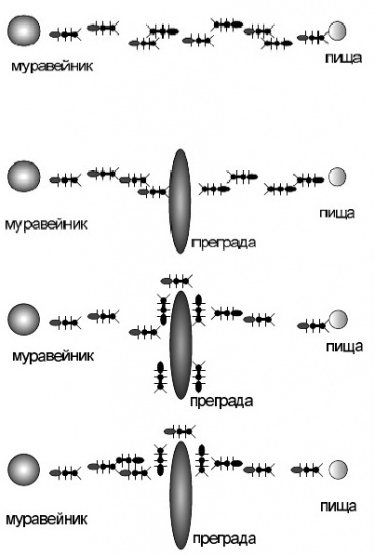
\includegraphics[scale=0.6]{images/pic_way.png}
		\caption{Схема движения муравьёв.}
		\label{fig:pic_way}
	\end{center}
\end{figure}

\section{Применение для задачи коммивояжёра}
Любой муравьиный алгоритм, независимо от модификаций, представим в следующем виде.
\begin{enumerate}
	\item  Создаем муравьёв.
	
	Стартовая точка, куда помещается муравей, зависит ограничений,   накладываемых условиями задачи. Потому что для каждой задачи   способ размещения муравьёв является определяющим. Либо все    они помещаются в одну точку, либо в разные с повторения, либо    без повторений. 
	
	На этом же этапе задается начальный уровень феромона. Он    инициализируется небольшим положительным числом для того,    чтобы на начальном шаге вероятности перехода в следующую вершину не были нулевыми. 
	
	\item Ищем решения.
	
	Вероятность перехода из вершины i в вершину j определяется по следующей формуле:\\   
	\begin{equation}
	P_{i j, k} (t)= \begin{cases}
	\displaystyle[\tau_{ij}(t)]^\alpha \cdot [\eta_{ij}]^\beta\over 
	\displaystyle\sum\limits_{l \in J_{i, k }} [\tau_{il}(t)]^\alpha \cdot \eta_{il}]^\beta  &,  j \in J_{i, k};\\
	0 &,  j \notin J_{i, k}
	\end{cases}
	\end{equation}
	\begin{align*}
	\text{где} \\
	\tau _{i,j} &- \text{ расстояние от города i до j;} \\
	\eta _{i,j} &- \text{ количество феромонов на ребре ij;} \\
	\alpha &- \text{параметр влияния длины пути;} \\
	\beta &- \text{параметр влияния феромона.}
	\end{align*}
	
	\item Обновляем феромон.
	
	Уровень феромона обновляется в соответствии с приведённой формулой:
	После того, как муравей успешно проходит маршрут, он оставляет на всех пройденных ребрах след, обратно пропорциональный длине пройденного пути:
	\begin{equation}\label{form:eva} 
	\tau _{i,j}=(1-\rho )\tau _{i,j}+\Delta \tau _{i,j},
	\end{equation}
	\begin{align*}
	\text{где} \\
	\rho _{i,j} &- \text{доля феромона, который испарится;} \\
	\tau _{i,j} &- \text{количество феромона на дуге ij;} \\
	\Delta \tau _{i,j} &- \text{количество отложенного феромона.}
	\end{align*}
	
	Также нужно заметить, что количество отложенного феромона ($\tau _{i,j}$) является суммой всех $\Delta \tau _{i,j}^k$:\\
	
	\begin{equation}\label{form:add} 
	{\displaystyle \Delta \tau _{i,j}^k={\begin{cases}Q/L_{k}& {\mbox{Если k-ый мурваей прошел по ребру ij;}}\\0&{\mbox{Иначе}}\end{cases}}}
	\end{equation}
	\begin{align*}
	\text{где} \\
	Q &- \text{количество феромона, переносимого муравьем;} \\
	L_{k} &- \text{стоимость k-го пути муравья (обычно длина).}
	\end{align*}  
	
\end{enumerate}

Теперь с учетом особенностей задачи коммивояжёра, мы можем описать локальные правила поведения муравьев при выборе пути.
\begin{enumerate}
	\item  Муравьи имеют собственную «память». Поскольку каждый город может быть посещён только один раз, то у каждого муравья есть список уже посещенных городов - список запретов. Обозначим через $J$ список городов, которые необходимо посетить муравью $k$ , находящемуся в городе $i$ .
	
	\item Муравьи обладают «зрением» - видимость есть эвристическое желание посетить город $j$ , если муравей находится в городе $i$ . Будем считать, что видимость обратно пропорциональна расстоянию между городами.
	
	\item Муравьи обладают «обонянием» - они могут улавливать след феромона, подтверждающий желание посетить город $j$ из города $i$ на основании опыта других муравьёв. Количество феромона на ребре $(i,j)$ в момент времени $t$ обозначим через  $tau _{i,j} (t)$.
	
	\item На этом основании мы можем сформулировать вероятностнопропорциональное правило, определяющее вероятность перехода $k$-ого муравья из города $i$  в город $j$.
	
	\item  Пройдя ребро $(i,j)$ , муравей откладывает на нём некоторое количество феромона, которое должно быть связано с оптимальностью сделанного выбора. Пусть $T _{k} (t)$ есть маршрут, пройденный муравьем $k$ к моменту времени $t$ , $L _{k} (t)$ - длина этого маршрута, а $Q$ - параметр, имеющий значение порядка длины оптимального пути~\cite{3}.
\end{enumerate} 

\section{Метод полного перебора.}

Метод полного перебора, по-другому именуемый методом грубой силы, является простым, логичным и широко используемым
математическим методом. Он применим во многих, если не во всех,
областях математики: задача коммивояжера также не является исключением.
Идея brute force предельно проста: перебираются всевозможные
решения и из них выбирается решение (или множество решений) отвечающее
условию задачи.

В задаче коммивояжера, соответственно, требуется из всевозможных
вариантов объезда пунктов выбрать маршрут, занимающий кратчайшее время
(или минимальный по стоимости маршрут).

Огромным преимуществом метода полного перебора перед другими
методами решения задачи коммивояжера является гарантированность
нахождения наилучшего маршрута. Другие методы советуют лишь
«хороший» маршрут, который совсем не обязательно является лучшим. Кроме
того, к достоинствам метода относится простота его программной реализации.

Однако, в связи с наличием огромного недостатка, метод полного
перебора крайне редко используется на практике. Этим недостатком является
временная сложность алгоритма. Асимметричная задача коммивояжера с n
посещаемых пунктов требует при полном переборе рассмотрения (n-1)! туров,
а факториал  растет невероятно быстро. Поэтому метод полного перебора может применяться только для задач
малой размерности (при рассмотрении до двух десятков посещаемых
пунктов) [4].

\section*{Вывод}

В данном разделе поставлена цель и описаны задачи описана теоретическая часть муравьиного алгоритма и полного перебора.
\newpage

\chapter{Конструкторская часть}
В данном разделе будет представлено описание архитектуры ПО и схемы  муравьинного алгоритма и алгоритма перебором.

\section{Требования к выводу}

Вывести таблицу с результатами параметризации. Столбцы: коэффициент либо жадности, либо стадности (второй из них не приводится, т.к. он связан с другим формулой), коэффициент испарения феромона, количество поколений ("суток" жизни колонии), значение длины лучшего найденного за 2-3 прогона муравьиного алгоритма пути и разность между этим значением и эталонным (по паре столбцов длина, разность длин на каждую "карту" класса данных). До таблицы приводят эталонные длины маршрутов, полученные методом полного перебора.

\section{Схемы алгоритмов.}

На рисунках \ref{fig:formic1}, \ref{fig:formic2}, \ref{fig:formic3} представлена схема муравьиного алгоритма.

\begin{figure}[H]
	\begin{center}
		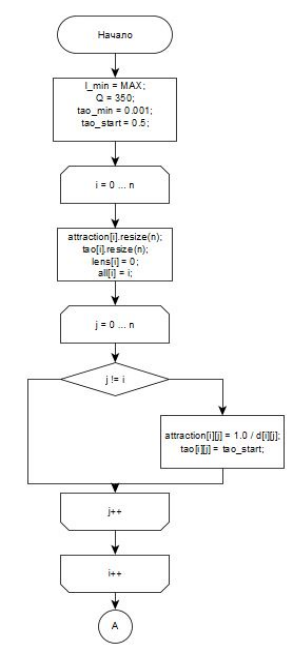
\includegraphics[scale=1]{images/formic.png}
		\caption{Схема муравьиного алгоритма часть 1.}
		\label{fig:formic1}
	\end{center}
\end{figure}

\begin{figure}[H]
	\begin{center}
		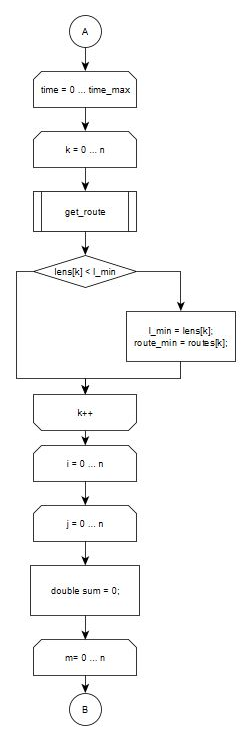
\includegraphics[scale=1]{images/formic2.png}
		\caption{Схема муравьиного алгоритма часть 2.}
		\label{fig:formic2}
	\end{center}
\end{figure}

\begin{figure}[H]
	\begin{center}
		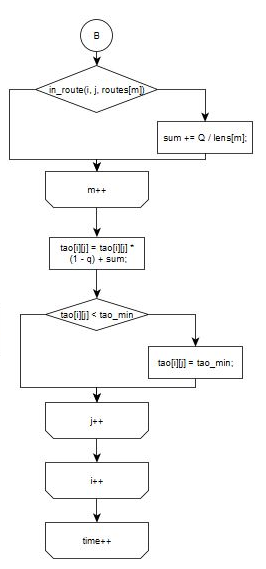
\includegraphics[scale=1]{images/formic3.png}
		\caption{Схема муравьиного алгоритма часть 3.}
		\label{fig:formic3}
	\end{center}
\end{figure}

На рисунках \ref{fig:en1}, \ref{fig:en2} представлена схема метода полного перебора.
\begin{figure}[H]
	\begin{center}
		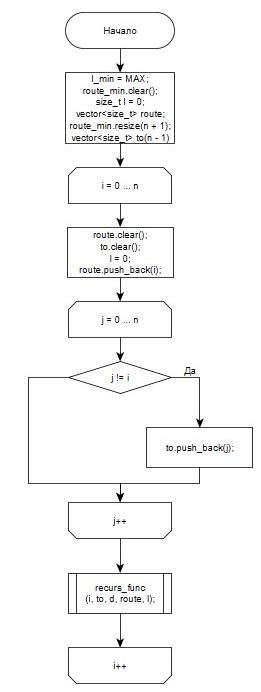
\includegraphics[scale=1]{images/enumeration1.png}
		\caption{Схема метода полного перебора часть 1.}
		\label{fig:en1}
	\end{center}
\end{figure}

\begin{figure}[H]
	\begin{center}
		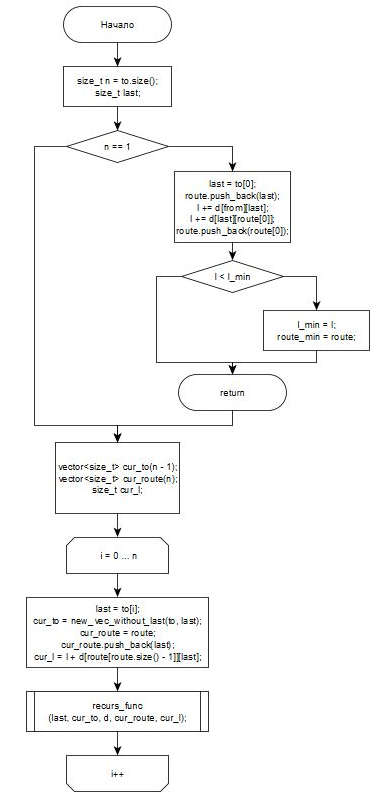
\includegraphics[scale=1]{images/enumeration2.png}
		\caption{Схема метода полного перебора часть 2.}
		\label{fig:en2}
	\end{center}
\end{figure}

\section*{Вывод}
В данном разделе представлено описание архитектуры ПО и схемы  муравьинного алгоритма и алгоритма перебором.

\chapter{Технологическая часть}
Данный раздел содержит обоснование выбора языка и среды разработки, реализацию алгоритмов.

\section{Средства реализации}
Для реализации программы был выбран язык программирования C++~\cite{}. Такой выбор обусловлен следующими причинами:
\begin{itemize}
	\item имеет высокую производительность;
	\item наличие библиотек для удобной работы с векторами и замеров времени.
\end{itemize}

Для замера времени выполнения использовалась функция $clock()$ из библиотеки ctime. Эта функция возвращает количество временных тактов, прошедших с начала запуска программы ~\cite{cpp}. 

\section{Реализация алгоритмов}
В листингах \ref{lst:det_rec} - \ref{lst:work_thread} представлены реализации рассматриваемых алгоритмов.
%\newpage
\captionsetup{singlelinecheck=false, justification=raggedright}
\begin{lstlisting}[label={lst:conv1},caption=Реализация алгоритма полного перебора.]
void recurs_func(size_t from, vector<size_t> to, vector<vector<size_t>> d, vector<size_t> route, size_t l) {

	size_t n = to.size();
	size_t last;
	if (n == 1) {
		last = to[0];
		route.push_back(last);
		l += d[from][last];
		l += d[last][route[0]];
		route.push_back(route[0]);
		if (l < l_min) {
			l_min = l;
			route_min = route;
		}
		return;
	}

	vector<size_t> cur_to(n - 1);
	vector<size_t> cur_route(n);
	size_t cur_l;
	for (size_t i = 0; i < n; i++) {
		last = to[i];
		cur_to = new_vec_without_last(to, last);
		cur_route = route;
		cur_route.push_back(last);
		cur_l = l + d[route[route.size() - 1]][last];
		recurs_func(last, cur_to, d, cur_route, cur_l);
	}

}

void perebor(size_t n, vector<vector<size_t>> d) {
	l_min = MAX;
	route_min.clear();
	size_t l = 0;
	vector<size_t> route;
	route_min.resize(n + 1);
	vector<size_t> to(n - 1);
	
	for (size_t i = 0; i < n; i++) {
		route.clear();
		to.clear();
		l = 0;
		
		route.push_back(i);
		for (size_t j = 0; j < n; j++)
			if (j != i)
				to.push_back(j);
		recurs_func(i, to, d, route, l);
	}
	
	cout << endl << "ROUTE: ";
	print_arr(route_min);
	cout << "LENGTH: " << l_min << endl << endl;
}
\end{lstlisting}


\begin{lstlisting}[label={lst:conv1},caption=Реализация муравьиного алгоритма.]
vector<double> get_probability(size_t from, vector<size_t> to, vector<vector<double>> tao, vector<vector<double>> attraction,
size_t alpha, size_t beta) {

	double znam = 0, chisl = 0;
	size_t n = to.size();
	vector<double> result(n);
	for (size_t i = 0; i < n; i++) {
		znam += pow(tao[from][to[i]], alpha) * pow(attraction[from][to[i]], beta);
	}
	for (size_t j = 0; j < n; j++) {
		chisl = pow(tao[from][to[j]], alpha) * pow(attraction[from][to[j]], beta);
		result[j] = chisl / znam;
	}
	return result;
}

void get_route(vector<size_t> all, size_t start, vector<size_t> &route, size_t &len, vector<vector<size_t>> d,
vector<vector<double>> tao, vector<vector<double>> attraction,
size_t alpha, size_t beta) {

	route.resize(0);
	route.push_back(start);
	vector<size_t> to = new_vec_without_last(all, start);
	size_t n_1 = tao.size() - 2;
	size_t from;
	double coin, sum;
	bool flag;
	
	for (size_t i = 0; i < n_1; i++) {
		sum = 0;
		flag = true;
		from = route[i];
		vector<double> p = get_probability(from, to, tao, attraction, alpha, beta);
		coin = double(rand() % 10000) / 10000;
		for (size_t j = 0; j < p.size() && flag; j++) {
			sum += p[j];
			if (coin < sum) {
				route.push_back(to[j]);
				len += d[from][to[j]];
				to = new_vec_without_last(to, to[j]);
				flag = false;
			}
		}
	}
	len += d[route[route.size() - 1]][to[0]];
	route.push_back(to[0]);
	len += d[route[route.size() - 1]][route[0]];
	route.push_back(route[0]);
}

void ant(size_t n, vector<vector<size_t>> d, size_t alpha, size_t beta, double q, size_t time_max, ofstream& file) {

	l_min = MAX;
	route_min.clear();
	
	double tao_min, tao_start, Q;
	vector<size_t> all(n);
	Q = 350;
	tao_min = 0.001;
	tao_start = 0.5;
	
	vector<vector<size_t>> routes(n);
	vector<size_t> lens(n);
	
	vector<vector<double>> attraction(n);
	vector<vector<double>> tao(n);
	
	for (size_t i = 0; i < n; i++) {
		attraction[i].resize(n);
		tao[i].resize(n);
		lens[i] = 0;
		all[i] = i;
		for (size_t j = 0; j < n; j++) {
			if (i != j) {
				attraction[i][j] = 1.0 / d[i][j];
				tao[i][j] = tao_start;
			}
		}
	}

	for (size_t time = 0; time < time_max; time++) {
		for (size_t k = 0; k < n; k++) {
			get_route(all, k, routes[k], lens[k], d, tao, attraction, alpha, beta);
			if (lens[k] < l_min) {
				l_min = lens[k];
				route_min = routes[k];
			}
		}
		for (size_t i = 0; i < n; i++)
			for (size_t j = 0; j < n; j++) {
				double sum = 0;
				for (size_t m = 0; m < n; m++) {
					if (in_route(i, j, routes[m]))
						sum += Q / lens[m];
					}
				
					tao[i][j] = tao[i][j] * (1 - q) + sum;
					if (tao[i][j] < tao_min)
						tao[i][j] = tao_min;
				}
			}
}
\end{lstlisting}

\section{Функциональные тесты}

В первом столбце таблицы \ref{tab3} представлена матрица расстояний, во втором - длина кратчайшего пути, в третьем найденная длина кратчайшего пути алгоритмом полного перебора. Путь найдённый алгоритмом полного перебора и результат выполнения муравьиного алгоритма представлены в приложении 1. 


\begin{table}[H]
	\caption{Функциональные тесты}
	\label{tab3}
	\begin{center}
		\begin{tabular}{ | c | c | c |}
			\hline
			\textbf{Матрица} & \textbf{Ожидаемая l} & \textbf{Фактическая l} \\ \hline
			$\begin{bmatrix} 
			0&1&3&2&1&3&2&4&1&2 \\
			1&0&1&3&2&1&2&1&1&2 \\
			3&1&0&1&2&1&1&2&3&1 \\
			2&3&1&0&1&2&1&2&1&1 \\
			1&2&2&1&0&2&2&1&2&2 \\
			3&1&1&2&2&0&1&1&2&1 \\
			2&2&1&1&2&1&0&3&2&3 \\
			4&1&2&2&1&2&3&0&1&4 \\
			1&1&3&1&2&2&2&1&0&1 \\
			2&2&1&1&2&1&3&4&1&0 \\
			
		\end{bmatrix}$ & 
		\text{10} 
		& 
		\text{ 10} \\
		
		\hline
		
	\end{tabular}
	
\end{center}
\end{table} 
Фактические результаты тестов совпали с ожидаемыми результатами.

\section*{Вывод}
В этом разделе обоснован выбор языка програмирования, описаны технические характеристики,приведены листинги кода реализованных алгоритмов и проведены тесты.
\newpage

\chapter{Экспериментальная часть}
В данном разделе сравниваются реализованные алгоритмы, дается сравнительная оценка затрат на время.

\section{Пример работы программы}
Пример работы программы представлен на рисунке \ref{fig:ex}. На вход подаётся файл с матрицей расстояний. Результат работы муравьиного алгоритма записывается в файл, один из вариантов выводится в консоль. Пример файла в приложении 1.
\captionsetup{singlelinecheck=true}
\begin{figure}[H]
	\centering
	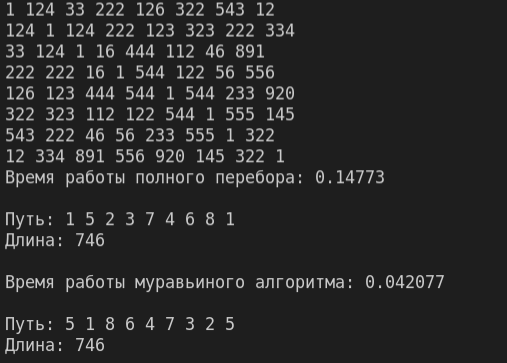
\includegraphics[width=1\linewidth]{images/ex}
	\caption{Пример работы программы}
	\label{fig:ex}
\end{figure}

\section{Технические характеристики}
Технические характеристики устройства, на котором выполнялось исследование:
\begin{itemize}
	\item операционная система: Ubuntu 20.01 Linux x86\_64~\cite{ubuntu};
	\item оперативная память: 8 Гб;
	\item процессор: AMD Ryzen5 4500U~\cite{processor}:
	\begin{itemize}
		\item количество физических ядер: 6;
		\item количество логических ядер: 6.
	\end{itemize}
\end{itemize}

\section{Время выполнения алгоритмов}
Был проведен сравнительный анализ реализаций муравьиного алгоритма и полного перебора. Замеры времени проводились для графов с количеством вершин от 2 до 10 с шагом 1. Значения коэффициентов составили $\alpha$ = 0, $t_{max}$ = 50, $\rho$ = 0.1.\\
Результаты представлены в таблице \ref{tab2}:\\

\begin{table}[H]
	\caption{Результаты замеров времени для алгоритма полного перебора и муравьиного алгоритма}
	\begin{center}
		\label{tab2}
		\begin{tabular}{|c|c|c|}
			\hline
			Количество вершин &Полный перебор& Муравьиный алгоритм \\\hline
			2&0.00001&0.00041\\
			3&0.00004&0.00096\\
			4&0.0002&0.002\\
			5&0.00053&0.0034\\
			6&0.0026&0.0062\\
			7&0.0175&0.0095\\
			8&0.13&0.013\\
			9&1.41&0.02\\
			10&14.88&0.027\\
			\hline
		\end{tabular}
	\end{center}
\end{table} 

\begin{center}
	\begin{tikzpicture}
	\begin{axis}[
	xlabel={Разница времени выполнения алгоритмов},
	ylabel={Время в секундах},
	xmin = 0, xmax = 10,
	ymin = 0, ymax = 20,
	legend pos=north west,
	ymajorgrids=true,
	grid style=dashed,
	]
	\legend{ 
		Алгоритм полного перебора,
		Муравьиный алгоритм
	}
	\addplot[
	color=yellow,
	mark=square,
	]
	coordinates {
		(2,  0.00001)
		(3,  0.00004)
		(4, 0.0002)
		(5, 0.00053)
		(6, 0.0026)
		(7, 0.0175)
		(8, 0.13)
		(9, 1.41)
		(10, 14.88)
	};
	\addplot[
	color=red,
	mark=square,
	]
	coordinates {
		(2,  0.00041)
		(3,  0.00096)
		(4, 0.002)
		(5, 0.0034)
		(6, 0.0062)
		(7, 0.0095)
		(8, 0.013)
		(9, 0.02)
		(10, 0.027)
	};
	\end{axis}
	\end{tikzpicture}
\end{center}

\section{Параметризация муравьиного алгоритма на основании проведенного эксперимента}	

Для различных значений параметров $\alpha$, $\beta$, $\rho$ и $t_{max}$ для каждой из нескольких матриц смежности с помощью муравьиного алгоритма и перебора была найдена некоторая длина маршрута. Далее выбраны наилучшие сочетания параметров муравьиного алгоритма на этих данных.\\
Параметр $\alpha$ менялся от 0 до 1 с шагом 0.25, параметр $\rho$ менялся от 0.1 до 0.9 с шагом 0.1, параметр $t_{max}$ менялся от 50 до 400 с шагом 50.\\
Были выявлены оптимальные сочетания параметров, представленные в таблице \ref{tab1}:\\

\begin{table}[H]
	\caption{Результаты решения задачи параметризации}
	\label{tab1}
	\begin{center}
		
		\begin{tabular}{|c|c|c|c|}
			\hline
			$\alpha$ &$\beta$ & $\rho$ & $t_{max}$ \\\hline
			4&6&0.6&20\\
			6&4&0.3&40\\
			1&9&0.7&50\\
			6&4&0.9&70\\
			3&7&0.6&80\\
			6&4&0.25&90\\
			\hline
		\end{tabular}
	\end{center}
\end{table} 

\section*{Вывод}
По результатам исследования муравьиный алгоритм при количестве вершин больше 6 выигрывает во времени выполнения у алгоритма полного перебора, поскольку время выполнения перебора очень быстро растет при увеличении числа вершин.\\

Для заданных классов данных найдены параметры, которые обеспечивают наиболее оптимальное решение.
\newpage

\addcontentsline{toc}{chapter}{Заключение}
\chapter*{Заключение}
В процессе выполнения лабораторной работы были изучены и реализованы алгоритмы последовательного и параллельного вычисления определителя квадратной матрицы.

Было исследовано время выполнения выше обозначенных алгоритмов. В результате было выявлено, что на матрицах, размер которых не превышает 5, использование параллельных вычислений нецелесообразно из-за превышения затратами на содержание потоков затрат на последовательное вычисление определителя. С увеличением размеров увеличивается эффективность использования параллельных вычислений, причем чем больше количество процессов, тем позже появляется выигрыш, но тем более существенным он оказывается. Исключением является использование 24 потоков в связи с увеличением затрат на обслуживание потоков в ядрах по сравнению с 16 потоками. Таким образом, выигрыш для 4 и 8 потоков проявляется на матрицах, больших $6\times6$ и составляет от 1.2 до 1.7 раз и от 1.2 до 2.8 раз соответственно, для восьми потоков - на матрицах, больших $7\times7$, от 1.5 до 3.5 раз, для 16 и 24 потоков - на матрицах, больших $8\times8$, от  2.7 до 4.4 раз и от 2.3 до 4.28 раз соответственно. Наиболее эффективным для матриц, больших $8\times8$, является использование 16 потоков, для матриц $7\times7$ - 8 потоков, $6\times6$ - четырех.

\newpage
\addcontentsline{toc}{chapter}{Список литературы}

\bibliographystyle{utf8gost705u}
\bibliography{bib_lab_4}
\nocite{*}

\newpage
\section*{Приложение 1. Результат работы алгоритма полного перебора и муравьиного алгоритма.}\addcontentsline{toc}{section}{Приложение}

Матрица расстояний:

$\begin{bmatrix} 
0&1&3&2&1&3&2&4&1&2 \\
1&0&1&3&2&1&2&1&1&2 \\
3&1&0&1&2&1&1&2&3&1 \\
2&3&1&0&1&2&1&2&1&1 \\
1&2&2&1&0&2&2&1&2&2 \\
3&1&1&2&2&0&1&1&2&1 \\
2&2&1&1&2&1&0&3&2&3 \\
4&1&2&2&1&2&3&0&1&4 \\
1&1&3&1&2&2&2&1&0&1 \\
2&2&1&1&2&1&3&4&1&0 \\

\end{bmatrix}$ 

Результат работы алгоритма полного перебора:

Путь: 1 2 3 4 7 6 10 9 8 5 1 

Длина: 10

Время работы: 25.2271

В листинге 1 выводится максимальное время  коэффициент жадности  коэффициент стадности коэффициент испарения ферoмона длина минимального пути путь. Длинной эталонного пути считается длина найденная алгоритмом полного перебора равная 10.
\chapter*{Приложение}
\addcontentsline{toc}{chapter}{Приложение}

\begin{table}[h]
\caption{Время (такт) выполнения полного перебора и муравьиного алгоритма}
\label{tbl:only}
\begin{center}
	\begin{tabular}{|c|c|c|c|c|c|c|}
		\hline
		$\alpha$ & $\beta$ & $\rho$ &  $t_{max}$ & $\Delta L_{1}$ & $\Delta L_{2}$ & $\Delta L_{3}$ \\
		\hline
		
		  50 & 0 & 1 & 0.1 & 346 & 3 & 115 \\
		 50 & 0 & 1 & 0.2 & 294 & 3 & 57 \\
		 50 & 0 & 1 & 0.3 & 518 & 3 & 48 \\
		 50 & 0 & 1 & 0.4 & 709 & 3 & 179 \\
		 50 & 0 & 1 & 0.5 & 283 & 1 & 86 \\
		 50 & 0 & 1 & 0.6 & 40 & 3 & 186 \\
		 50 & 0 & 1 & 0.7 & 684 & 1 & 55 \\
		 50 & 0 & 1 & 0.8 & 546 & 2 & 184 \\
		 50 & 0 & 1 & 0.9 & 306 & 4 & 88 \\
		 50 & 0.25 & 0.75 & 0.1 & 1527 & 5 & 194 \\
		 50 & 0.25 & 0.75 & 0.2 & 1399 & 5 & 315 \\
		 50 & 0.25 & 0.75 & 0.3 & 822 & 5 & 370 \\
		 50 & 0.25 & 0.75 & 0.4 & 1069 & 6 & 350 \\
		 50 & 0.25 & 0.75 & 0.5 & 1193 & 3 & 351 \\
		 50 & 0.25 & 0.75 & 0.6 & 984 & 6 & 310 \\
		 50 & 0.25 & 0.75 & 0.7 & 1224 & 5 & 443 \\
		 50 & 0.25 & 0.75 & 0.8 & 1546 & 4 & 486 \\
		 50 & 0.25 & 0.75 & 0.9 & 767 & 0 & 355 \\
		 50 & 0.5 & 0.5 & 0.1 & 1295 & 3 & 251 \\
		 50 & 0.5 & 0.5 & 0.2 & 1426 & 2 & 354 \\
		 50 & 0.5 & 0.5 & 0.3 & 892 & 5 & 90 \\
		 50 & 0.5 & 0.5 & 0.4 & 323 & 4 & 370 \\
		 50 & 0.5 & 0.5 & 0.5 & 923 & 5 & 392 \\
		 50 & 0.5 & 0.5 & 0.6 & 989 & 4 & 446 \\
		 50 & 0.5 & 0.5 & 0.7 & 1480 & 4 & 298 \\
		 50 & 0.5 & 0.5 & 0.8 & 995 & 4 & 358 \\
		 50 & 0.5 & 0.5 & 0.9 & 1467 & 4 & 388 \\
		 50 & 0.75 & 0.25 & 0.1 & 840 & 3 & 327 \\
		 50 & 0.75 & 0.25 & 0.2 & 1466 & 6 & 203 \\
		 50 & 0.75 & 0.25 & 0.3 & 1513 & 2 & 408 \\
		 50 & 0.75 & 0.25 & 0.4 & 1318 & 2 & 317 \\
		 50 & 0.75 & 0.25 & 0.5 & 1533 & 3 & 344 \\
		 50 & 0.75 & 0.25 & 0.6 & 760 & 6 & 315 \\
		 50 & 0.75 & 0.25 & 0.7 & 1514 & 2 & 315 \\
		 50 & 0.75 & 0.25 & 0.8 & 661 & 5 & 361 \\
		 50 & 0.75 & 0.25 & 0.9 & 1309 & 4 & 275 \\
		 50 & 1 & 0 & 0.1 & 1452 & 5 & 306 \\
		 50 & 1 & 0 & 0.2 & 1326 & 4 & 209 \\
		 50 & 1 & 0 & 0.3 & 1523 & 5 & 328 \\
		 \hline
	\end{tabular}
\end{center}
\end{table}
\newpage 

\begin{table}[h]
\caption{Время (такт) выполнения полного перебора и муравьиного алгоритма}
\label{tbl:only}
\begin{center}
	\begin{tabular}{|c|c|c|c|c|c|c|}
		\hline
		$\alpha$ & $\beta$ & $\rho$ &  $t_{max}$ & $\Delta L_{1}$ & $\Delta L_{2}$ & $\Delta L_{3}$\\
		\hline
		50 & 1 & 0 & 0.4 & 1761 & 3 & 397 \\
		50 & 1 & 0 & 0.5 & 1897 & 5 & 283 \\
		50 & 1 & 0 & 0.6 & 1605 & 6 & 322 \\
		50 & 1 & 0 & 0.7 & 1833 & 3 & 322 \\
		50 & 1 & 0 & 0.8 & 764 & 5 & 399 \\
		50 & 1 & 0 & 0.9 & 1479 & 3 & 433 \\
		100 & 0 & 1 & 0.1 & 235 & 1 & 175 \\
		100 & 0 & 1 & 0.2 & 283 & 2 & 100 \\
		100 & 0 & 1 & 0.3 & 92 & 2 & 146 \\
		100 & 0 & 1 & 0.4 & 40 & 1 & 67 \\
		100 & 0 & 1 & 0.5 & 576 & 3 & 123 \\
		100 & 0 & 1 & 0.6 & 282 & 3 & 135 \\
		100 & 0 & 1 & 0.7 & 277 & 2 & 135 \\
		100 & 0 & 1 & 0.8 & 555 & 2 & 4 \\
		100 & 0 & 1 & 0.9 & 85 & 2 & 120 \\
		100 & 0.25 & 0.75 & 0.1 & 779 & 5 & 192 \\
		100 & 0.25 & 0.75 & 0.2 & 1124 & 6 & 320 \\
		100 & 0.25 & 0.75 & 0.3 & 1262 & 3 & 428 \\
		100 & 0.25 & 0.75 & 0.4 & 867 & 4 & 297 \\
		100 & 0.25 & 0.75 & 0.5 & 1890 & 3 & 153 \\
		100 & 0.25 & 0.75 & 0.6 & 1242 & 3 & 222 \\
		100 & 0.25 & 0.75 & 0.7 & 1532 & 5 & 424 \\
		100 & 0.25 & 0.75 & 0.8 & 521 & 5 & 268 \\
		100 & 0.25 & 0.75 & 0.9 & 1977 & 2 & 243 \\
		100 & 0.5 & 0.5 & 0.1 & 1905 & 3 & 260 \\
		100 & 0.5 & 0.5 & 0.2 & 1809 & 6 & 255 \\
		100 & 0.5 & 0.5 & 0.3 & 1233 & 4 & 457 \\
		100 & 0.5 & 0.5 & 0.4 & 1355 & 3 & 362 \\
		100 & 0.5 & 0.5 & 0.5 & 897 & 4 & 103 \\
		100 & 0.5 & 0.5 & 0.6 & 1135 & 4 & 227 \\
		100 & 0.5 & 0.5 & 0.7 & 1237 & 2 & 332 \\
		100 & 0.5 & 0.5 & 0.8 & 565 & 3 & 46 \\
		100 & 0.5 & 0.5 & 0.9 & 1934 & 3 & 168 \\
		100 & 0.75 & 0.25 & 0.1 & 1176 & 3 & 267 \\
		100 & 0.75 & 0.25 & 0.2 & 2140 & 5 & 384 \\
		100 & 0.75 & 0.25 & 0.3 & 1542 & 6 & 253 \\
		100 & 0.75 & 0.25 & 0.4 & 1200 & 4 & 163 \\
		100 & 0.75 & 0.25 & 0.5 & 1163 & 4 & 223 \\
		100 & 0.75 & 0.25 & 0.6 & 1743 & 4 & 452 \\
		\hline
		
	\end{tabular}
\end{center}
\end{table}
\begin{table}[h]
\caption{Время (такт) выполнения полного перебора и муравьиного алгоритма}
\label{tbl:only}
\begin{center}
	\begin{tabular}{|c|c|c|c|c|c|c|}
		\hline
		$\alpha$ &  $\beta$& $\rho$ &  $t_{max}$ & $\Delta L_{1}$ & $\Delta L_{2}$ & $\Delta L_{3}$\\
		\hline
		100 & 0.75 & 0.25 & 0.7 & 867 & 4 & 151 \\
		100 & 0.75 & 0.25 & 0.8 & 1268 & 5 & 338 \\
		100 & 0.75 & 0.25 & 0.9 & 1119 & 4 & 327 \\
		100 & 1 & 0 & 0.1 & 836 & 2 & 398 \\
		100 & 1 & 0 & 0.2 & 789 & 4 & 279 \\
		100 & 1 & 0 & 0.3 & 684 & 4 & 258 \\
		100 & 1 & 0 & 0.4 & 1494 & 5 & 438 \\
		100 & 1 & 0 & 0.5 & 1230 & 3 & 247 \\
		100 & 1 & 0 & 0.6 & 933 & 4 & 272 \\
		100 & 1 & 0 & 0.7 & 1089 & 3 & 328 \\
		100 & 1 & 0 & 0.8 & 1629 & 2 & 387 \\
		100 & 1 & 0 & 0.9 & 1041 & 3 & 376 \\
		150 & 0 & 1 & 0.1 & 120 & 3 & 248 \\
		150 & 0 & 1 & 0.2 & 529 & 2 & 235 \\
		150 & 0 & 1 & 0.3 & 592 & 1 & 208 \\
		150 & 0 & 1 & 0.4 & 282 & 3 & 142 \\
		150 & 0 & 1 & 0.5 & 297 & 2 & 68 \\
		150 & 0 & 1 & 0.6 & 379 & 5 & 47 \\
		150 & 0 & 1 & 0.7 & 488 & 4 & 49 \\
		150 & 0 & 1 & 0.8 & 282 & 2 & 123 \\
		150 & 0 & 1 & 0.9 & 502 & 1 & 201 \\
		150 & 0.25 & 0.75 & 0.1 & 899 & 5 & 371 \\
		150 & 0.25 & 0.75 & 0.2 & 1014 & 1 & 385 \\
		150 & 0.25 & 0.75 & 0.3 & 1775 & 5 & 197 \\
		150 & 0.25 & 0.75 & 0.4 & 1355 & 4 & 350 \\
		150 & 0.25 & 0.75 & 0.5 & 1403 & 5 & 335 \\
		150 & 0.25 & 0.75 & 0.6 & 516 & 3 & 347 \\
		150 & 0.25 & 0.75 & 0.7 & 1727 & 6 & 351 \\
		150 & 0.25 & 0.75 & 0.8 & 682 & 4 & 352 \\
		150 & 0.25 & 0.75 & 0.9 & 1197 & 4 & 432 \\
		150 & 0.5 & 0.5 & 0.1 & 887 & 7 & 254 \\
		150 & 0.5 & 0.5 & 0.2 & 1088 & 3 & 341 \\
		150 & 0.5 & 0.5 & 0.3 & 697 & 4 & 356 \\
		150 & 0.5 & 0.5 & 0.4 & 1401 & 6 & 243 \\
		150 & 0.5 & 0.5 & 0.5 & 921 & 5 & 333 \\
		150 & 0.5 & 0.5 & 0.6 & 1385 & 2 & 208 \\
		150 & 0.5 & 0.5 & 0.7 & 1281 & 6 & 254 \\
		150 & 0.5 & 0.5 & 0.8 & 1288 & 5 & 281 \\
		150 & 0.5 & 0.5 & 0.9 & 1029 & 3 & 318 \\
		\hline
		
	\end{tabular}
\end{center}
\end{table}
\begin{table}[h]
\caption{Время (такт) выполнения полного перебора и муравьиного алгоритма}
\label{tbl:only}
\begin{center}
	\begin{tabular}{|c|c|c|c|c|c|c|}
		\hline
		$\alpha$ & $\beta$ &$\rho$ &  $t_{max}$ & $\Delta L_{1}$ & $\Delta L_{2}$ & $\Delta L_{3}$\\
		\hline
		150 & 0.75 & 0.25 & 0.1 & 1382 & 4 & 399 \\
		150 & 0.75 & 0.25 & 0.2 & 1294 & 3 & 346 \\
		150 & 0.75 & 0.25 & 0.3 & 1359 & 3 & 176 \\
		150 & 0.75 & 0.25 & 0.4 & 1306 & 4 & 228 \\
		150 & 0.75 & 0.25 & 0.5 & 1716 & 4 & 417 \\
		150 & 0.75 & 0.25 & 0.6 & 1309 & 4 & 148 \\
		150 & 0.75 & 0.25 & 0.7 & 1002 & 4 & 478 \\
		150 & 0.75 & 0.25 & 0.8 & 1053 & 3 & 196 \\
		150 & 0.75 & 0.25 & 0.9 & 1292 & 5 & 397 \\
		150 & 1 & 0 & 0.1 & 1740 & 6 & 196 \\
		150 & 1 & 0 & 0.2 & 1074 & 5 & 455 \\
		150 & 1 & 0 & 0.3 & 1379 & 2 & 307 \\
		150 & 1 & 0 & 0.4 & 1350 & 0 & 371 \\
		150 & 1 & 0 & 0.5 & 1267 & 5 & 278 \\
		150 & 1 & 0 & 0.6 & 1796 & 3 & 321 \\
		150 & 1 & 0 & 0.7 & 1275 & 3 & 302 \\
		150 & 1 & 0 & 0.8 & 902 & 6 & 375 \\
		150 & 1 & 0 & 0.9 & 1421 & 4 & 239 \\
		200 & 0 & 1 & 0.1 & 413 & 2 & 303 \\
		200 & 0 & 1 & 0.2 & 573 & 0 & 30 \\
		200 & 0 & 1 & 0.3 & 661 & 3 & 17 \\
		200 & 0 & 1 & 0.4 & 624 & 2 & 130 \\
		200 & 0 & 1 & 0.5 & 678 & 2 & 152 \\
		200 & 0 & 1 & 0.6 & 578 & 3 & 37 \\
		200 & 0 & 1 & 0.7 & 510 & 1 & 102 \\
		200 & 0 & 1 & 0.8 & 389 & 3 & 164 \\
		200 & 0 & 1 & 0.9 & 521 & 2 & 215 \\
		200 & 0.25 & 0.75 & 0.1 & 1069 & 2 & 328 \\
		200 & 0.25 & 0.75 & 0.2 & 1137 & 5 & 388 \\
		200 & 0.25 & 0.75 & 0.3 & 1891 & 5 & 395 \\
		200 & 0.25 & 0.75 & 0.4 & 914 & 2 & 217 \\
		200 & 0.25 & 0.75 & 0.5 & 953 & 5 & 425 \\
		200 & 0.25 & 0.75 & 0.6 & 1361 & 4 & 267 \\
		200 & 0.25 & 0.75 & 0.7 & 1317 & 4 & 312 \\
		200 & 0.25 & 0.75 & 0.8 & 600 & 3 & 169 \\
		200 & 0.25 & 0.75 & 0.9 & 826 & 3 & 312 \\
		200 & 0.5 & 0.5 & 0.1 & 1116 & 4 & 303 \\
		200 & 0.5 & 0.5 & 0.2 & 1513 & 4 & 457 \\
		200 & 0.5 & 0.5 & 0.3 & 1230 & 3 & 307 \\
		\hline	
	\end{tabular}
\end{center}
\end{table}
\begin{table}[h]
\caption{Время (такт) выполнения полного перебора и муравьиного алгоритма}
\label{tbl:only}
\begin{center}
	\begin{tabular}{|c|c|c|c|c|c|c|}
		\hline
		$\alpha$ & $\beta$ & $\rho$ &  $t_{max}$ & $\Delta L_{1}$ & $\Delta L_{2}$ & $\Delta L_{3}$\\
		\hline
		200 & 0.5 & 0.5 & 0.4 & 1501 & 6 & 352 \\
		200 & 0.5 & 0.5 & 0.5 & 1508 & 4 & 304 \\
		200 & 0.5 & 0.5 & 0.6 & 1397 & 3 & 307 \\
		200 & 0.5 & 0.5 & 0.7 & 1340 & 2 & 360 \\
		200 & 0.5 & 0.5 & 0.8 & 544 & 5 & 161 \\
		200 & 0.5 & 0.5 & 0.9 & 1647 & 4 & 386 \\
		200 & 0.75 & 0.25 & 0.1 & 1551 & 2 & 293 \\
		200 & 0.75 & 0.25 & 0.2 & 868 & 5 & 212 \\
		200 & 0.75 & 0.25 & 0.3 & 890 & 2 & 399 \\
		200 & 0.75 & 0.25 & 0.4 & 1044 & 5 & 427 \\
		200 & 0.75 & 0.25 & 0.5 & 1514 & 4 & 297 \\
		200 & 0.75 & 0.25 & 0.6 & 1134 & 2 & 298 \\
		200 & 0.75 & 0.25 & 0.7 & 1879 & 4 & 291 \\
		200 & 0.75 & 0.25 & 0.8 & 1397 & 5 & 296 \\
		200 & 0.75 & 0.25 & 0.9 & 908 & 3 & 341 \\
		200 & 1 & 0 & 0.1 & 962 & 6 & 435 \\
		200 & 1 & 0 & 0.2 & 1361 & 4 & 300 \\
		200 & 1 & 0 & 0.3 & 671 & 4 & 334 \\
		200 & 1 & 0 & 0.4 & 686 & 3 & 384 \\
		200 & 1 & 0 & 0.5 & 1341 & 4 & 298 \\
		200 & 1 & 0 & 0.6 & 822 & 3 & 271 \\
		200 & 1 & 0 & 0.7 & 869 & 5 & 307 \\
		200 & 1 & 0 & 0.8 & 969 & 5 & 247 \\
		200 & 1 & 0 & 0.9 & 1290 & 4 & 251 \\
		250 & 0 & 1 & 0.1 & 488 & 1 & 120 \\
		250 & 0 & 1 & 0.2 & 277 & 2 & 47 \\
		250 & 0 & 1 & 0.3 & 455 & 2 & 121 \\
		250 & 0 & 1 & 0.4 & 348 & 4 & 125 \\
		250 & 0 & 1 & 0.5 & 235 & 2 & 194 \\
		250 & 0 & 1 & 0.6 & 235 & 4 & 140 \\
		250 & 0 & 1 & 0.7 & 211 & 1 & 4 \\
		250 & 0 & 1 & 0.8 & 423 & 2 & 66 \\
		250 & 0 & 1 & 0.9 & 501 & 3 & 190 \\
		250 & 0.25 & 0.75 & 0.1 & 961 & 2 & 259 \\
		250 & 0.25 & 0.75 & 0.2 & 1346 & 3 & 375 \\
		250 & 0.25 & 0.75 & 0.3 & 1483 & 4 & 360 \\
		250 & 0.25 & 0.75 & 0.4 & 661 & 2 & 353 \\
		250 & 0.25 & 0.75 & 0.5 & 1477 & 2 & 257 \\
		250 & 0.25 & 0.75 & 0.6 & 865 & 4 & 412 \\
		\hline
	\end{tabular}
\end{center}
\end{table}
\begin{table}[h]
\caption{Время (такт) выполнения полного перебора и муравьиного алгоритма}
\label{tbl:only}
\begin{center}
	\begin{tabular}{|c|c|c|c|c|c|c|}
		\hline
		$\alpha$ &  $\beta$&$\rho$ &  $t_{max}$ & $\Delta L_{1}$ & $\Delta L_{2}$ & $\Delta L_{3}$\\
		\hline
		250 & 0.25 & 0.75 & 0.7 & 1631 & 4 & 363 \\
		250 & 0.25 & 0.75 & 0.8 & 1848 & 4 & 322 \\
		250 & 0.25 & 0.75 & 0.9 & 934 & 5 & 526 \\
		250 & 0.5 & 0.5 & 0.1 & 1271 & 4 & 116 \\
		250 & 0.5 & 0.5 & 0.2 & 765 & 4 & 260 \\
		250 & 0.5 & 0.5 & 0.3 & 1978 & 5 & 365 \\
		250 & 0.5 & 0.5 & 0.4 & 1420 & 4 & 260 \\
		250 & 0.5 & 0.5 & 0.5 & 1048 & 6 & 356 \\
		250 & 0.5 & 0.5 & 0.6 & 1719 & 4 & 393 \\
		250 & 0.5 & 0.5 & 0.7 & 1967 & 3 & 256 \\
		250 & 0.5 & 0.5 & 0.8 & 1543 & 3 & 195 \\
		250 & 0.5 & 0.5 & 0.9 & 1207 & 5 & 282 \\
		250 & 0.75 & 0.25 & 0.1 & 1484 & 2 & 240 \\
		250 & 0.75 & 0.25 & 0.2 & 1385 & 3 & 316 \\
		250 & 0.75 & 0.25 & 0.3 & 508 & 1 & 294 \\
		250 & 0.75 & 0.25 & 0.4 & 1774 & 2 & 358 \\
		250 & 0.75 & 0.25 & 0.5 & 888 & 5 & 232 \\
		250 & 0.75 & 0.25 & 0.6 & 1455 & 3 & 225 \\
		250 & 0.75 & 0.25 & 0.7 & 1189 & 5 & 375 \\
		250 & 0.75 & 0.25 & 0.8 & 1103 & 4 & 183 \\
		250 & 0.75 & 0.25 & 0.9 & 1042 & 3 & 355 \\
		250 & 1 & 0 & 0.1 & 1398 & 3 & 148 \\
		250 & 1 & 0 & 0.2 & 1666 & 4 & 202 \\
		250 & 1 & 0 & 0.3 & 1014 & 3 & 288 \\
		250 & 1 & 0 & 0.4 & 1083 & 4 & 128 \\
		250 & 1 & 0 & 0.5 & 1137 & 5 & 211 \\
		250 & 1 & 0 & 0.6 & 1708 & 4 & 238 \\
		250 & 1 & 0 & 0.7 & 1432 & 3 & 299 \\
		250 & 1 & 0 & 0.8 & 1254 & 3 & 428 \\
		250 & 1 & 0 & 0.9 & 1510 & 3 & 287 \\
		300 & 0 & 1 & 0.1 & 654 & 1 & 128 \\
		300 & 0 & 1 & 0.2 & 412 & 2 & 46 \\
		300 & 0 & 1 & 0.3 & 85 & 3 & 164 \\
		300 & 0 & 1 & 0.4 & 488 & 0 & 69 \\
		300 & 0 & 1 & 0.5 & 402 & 3 & 134 \\
		300 & 0 & 1 & 0.6 & 133 & 2 & 107 \\
		300 & 0 & 1 & 0.7 & 704 & 1 & 179 \\
		300 & 0 & 1 & 0.8 & 606 & 2 & 31 \\
		300 & 0 & 1 & 0.9 & 313 & 2 & 161 \\
		\hline	
	\end{tabular}
\end{center}
\end{table}
\begin{table}[h]
\caption{Время (такт) выполнения полного перебора и муравьиного алгоритма}
\label{tbl:only}
\begin{center}
	\begin{tabular}{|c|c|c|c|c|c|c|}
		\hline
		$\alpha$ & $\beta$ &$\rho$ &  $t_{max}$ & $\Delta L_{1}$ & $\Delta L_{2}$ & $\Delta L_{3}$\\
		\hline
		300 & 0.25 & 0.75 & 0.1 & 1297 & 3 & 421 \\
		300 & 0.25 & 0.75 & 0.2 & 1577 & 6 & 305 \\
		300 & 0.25 & 0.75 & 0.3 & 902 & 3 & 453 \\
		300 & 0.25 & 0.75 & 0.4 & 1311 & 3 & 270 \\
		300 & 0.25 & 0.75 & 0.5 & 277 & 4 & 366 \\
		300 & 0.25 & 0.75 & 0.6 & 1689 & 5 & 333 \\
		300 & 0.25 & 0.75 & 0.7 & 234 & 5 & 15 \\
		300 & 0.25 & 0.75 & 0.8 & 1521 & 4 & 226 \\
		300 & 0.25 & 0.75 & 0.9 & 1223 & 4 & 340 \\
		300 & 0.5 & 0.5 & 0.1 & 1295 & 4 & 234 \\
		300 & 0.5 & 0.5 & 0.2 & 1857 & 3 & 365 \\
		300 & 0.5 & 0.5 & 0.3 & 1781 & 4 & 388 \\
		300 & 0.5 & 0.5 & 0.4 & 935 & 6 & 322 \\
		300 & 0.5 & 0.5 & 0.5 & 1003 & 4 & 395 \\
		300 & 0.5 & 0.5 & 0.6 & 1102 & 3 & 260 \\
		300 & 0.5 & 0.5 & 0.7 & 297 & 4 & 86 \\
		300 & 0.5 & 0.5 & 0.8 & 1524 & 4 & 425 \\
		300 & 0.5 & 0.5 & 0.9 & 1302 & 3 & 434 \\
		300 & 0.75 & 0.25 & 0.1 & 588 & 5 & 318 \\
		300 & 0.75 & 0.25 & 0.2 & 1552 & 5 & 445 \\
		300 & 0.75 & 0.25 & 0.3 & 1570 & 6 & 326 \\
		300 & 0.75 & 0.25 & 0.4 & 1307 & 3 & 309 \\
		300 & 0.75 & 0.25 & 0.5 & 1522 & 6 & 319 \\
		300 & 0.75 & 0.25 & 0.6 & 405 & 3 & 283 \\
		300 & 0.75 & 0.25 & 0.7 & 1047 & 5 & 401 \\
		300 & 0.75 & 0.25 & 0.8 & 1507 & 3 & 380 \\
		300 & 0.75 & 0.25 & 0.9 & 897 & 2 & 299 \\
		300 & 1 & 0 & 0.1 & 761 & 4 & 459 \\
		300 & 1 & 0 & 0.2 & 1419 & 5 & 230 \\
		300 & 1 & 0 & 0.3 & 1519 & 4 & 72 \\
		300 & 1 & 0 & 0.4 & 696 & 3 & 177 \\
		300 & 1 & 0 & 0.5 & 1423 & 5 & 289 \\
		300 & 1 & 0 & 0.6 & 1600 & 6 & 335 \\
		300 & 1 & 0 & 0.7 & 1043 & 4 & 280 \\
		300 & 1 & 0 & 0.8 & 1315 & 4 & 283 \\
		300 & 1 & 0 & 0.9 & 1005 & 4 & 407 \\
		350 & 0 & 1 & 0.1 & 726 & 3 & 170 \\
		350 & 0 & 1 & 0.2 & 339 & 2 & 113 \\
		350 & 0 & 1 & 0.3 & 322 & 1 & 74 \\	
		\hline
	\end{tabular}
\end{center}
\end{table}
\begin{table}[h]
\caption{Время (такт) выполнения полного перебора и муравьиного алгоритма}
\label{tbl:only}
\begin{center}
	\begin{tabular}{|c|c|c|c|c|c|c|}
		\hline
		$\alpha$ & $\beta$ & $\rho$ &  $t_{max}$ & $\Delta L_{1}$ & $\Delta L_{2}$ & $\Delta L_{3}$\\
		\hline
		350 & 0 & 1 & 0.4 & 437 & 2 & 100 \\
		350 & 0 & 1 & 0.5 & 404 & 3 & 64 \\
		350 & 0 & 1 & 0.6 & 34 & 1 & 54 \\
		350 & 0 & 1 & 0.7 & 247 & 3 & 165 \\
		350 & 0 & 1 & 0.8 & 303 & 1 & 258 \\
		350 & 0 & 1 & 0.9 & 120 & 4 & 11 \\
		350 & 0.25 & 0.75 & 0.1 & 1354 & 5 & 197 \\
		350 & 0.25 & 0.75 & 0.2 & 1358 & 4 & 418 \\
		350 & 0.25 & 0.75 & 0.3 & 1784 & 3 & 244 \\
		350 & 0.25 & 0.75 & 0.4 & 1148 & 2 & 246 \\
		350 & 0.25 & 0.75 & 0.5 & 1600 & 4 & 311 \\
		350 & 0.25 & 0.75 & 0.6 & 1435 & 6 & 426 \\
		350 & 0.25 & 0.75 & 0.7 & 1519 & 6 & 247 \\
		350 & 0.25 & 0.75 & 0.8 & 1013 & 3 & 211 \\
		350 & 0.25 & 0.75 & 0.9 & 956 & 5 & 244 \\
		350 & 0.5 & 0.5 & 0.1 & 1154 & 4 & 300 \\
		350 & 0.5 & 0.5 & 0.2 & 1584 & 5 & 389 \\
		350 & 0.5 & 0.5 & 0.3 & 1711 & 4 & 408 \\
		350 & 0.5 & 0.5 & 0.4 & 912 & 4 & 216 \\
		350 & 0.5 & 0.5 & 0.5 & 1822 & 5 & 290 \\
		350 & 0.5 & 0.5 & 0.6 & 1314 & 4 & 219 \\
		350 & 0.5 & 0.5 & 0.7 & 1898 & 5 & 332 \\
		350 & 0.5 & 0.5 & 0.8 & 1112 & 2 & 392 \\
		350 & 0.5 & 0.5 & 0.9 & 1499 & 3 & 223 \\
		350 & 0.75 & 0.25 & 0.1 & 1715 & 3 & 249 \\
		350 & 0.75 & 0.25 & 0.2 & 1982 & 5 & 363 \\
		350 & 0.75 & 0.25 & 0.3 & 1564 & 3 & 295 \\
		350 & 0.75 & 0.25 & 0.4 & 1288 & 5 & 400 \\
		350 & 0.75 & 0.25 & 0.5 & 914 & 4 & 285 \\
		350 & 0.75 & 0.25 & 0.6 & 1040 & 2 & 275 \\
		350 & 0.75 & 0.25 & 0.7 & 1484 & 6 & 418 \\
		350 & 0.75 & 0.25 & 0.8 & 1100 & 2 & 492 \\
		350 & 0.75 & 0.25 & 0.9 & 1550 & 4 & 447 \\
		350 & 1 & 0 & 0.1 & 1712 & 5 & 314 \\
		350 & 1 & 0 & 0.2 & 769 & 3 & 404 \\
		350 & 1 & 0 & 0.3 & 2358 & 5 & 405 \\
		350 & 1 & 0 & 0.4 & 1531 & 6 & 345 \\
		350 & 1 & 0 & 0.5 & 1229 & 3 & 308 \\
		350 & 1 & 0 & 0.6 & 779 & 4 & 277 \\
		\hline	
	\end{tabular}
\end{center}
\end{table}
\begin{table}[h]
\caption{Время (такт) выполнения полного перебора и муравьиного алгоритма}
\label{tbl:only}
\begin{center}
	\begin{tabular}{|c|c|c|c|c|c|c|}
		\hline
		$\alpha$ & $\beta$ &$\rho$ &  $t_{max}$ & $\Delta L_{1}$ & $\Delta L_{2}$ & $\Delta L_{3}$\\
		\hline
		350 & 1 & 0 & 0.7 & 1347 & 6 & 295 \\
		350 & 1 & 0 & 0.8 & 1350 & 1 & 331 \\
		350 & 1 & 0 & 0.9 & 1413 & 4 & 208 \\
		400 & 0 & 1 & 0.1 & 429 & 1 & 285 \\
		400 & 0 & 1 & 0.2 & 991 & 2 & 125 \\
		400 & 0 & 1 & 0.3 & 506 & 2 & 45 \\
		400 & 0 & 1 & 0.4 & 85 & 3 & 37 \\
		400 & 0 & 1 & 0.5 & 912 & 1 & 66 \\
		400 & 0 & 1 & 0.6 & 297 & 1 & 54 \\
		400 & 0 & 1 & 0.7 & 447 & 2 & 92 \\
		400 & 0 & 1 & 0.8 & 40 & 3 & 169 \\
		400 & 0 & 1 & 0.9 & 413 & 2 & 200 \\
		400 & 0.25 & 0.75 & 0.1 & 742 & 4 & 325 \\
		400 & 0.25 & 0.75 & 0.2 & 1924 & 2 & 347 \\
		400 & 0.25 & 0.75 & 0.3 & 578 & 4 & 368 \\
		400 & 0.25 & 0.75 & 0.4 & 1746 & 3 & 223 \\
		400 & 0.25 & 0.75 & 0.5 & 1306 & 2 & 365 \\
		400 & 0.25 & 0.75 & 0.6 & 802 & 4 & 192 \\
		400 & 0.25 & 0.75 & 0.7 & 965 & 4 & 309 \\
		400 & 0.25 & 0.75 & 0.8 & 1447 & 7 & 320 \\
		400 & 0.25 & 0.75 & 0.9 & 644 & 5 & 311 \\
		400 & 0.5 & 0.5 & 0.1 & 952 & 5 & 464 \\
		400 & 0.5 & 0.5 & 0.2 & 1177 & 3 & 163 \\
		400 & 0.5 & 0.5 & 0.3 & 797 & 5 & 386 \\
		400 & 0.5 & 0.5 & 0.4 & 929 & 5 & 316 \\
		400 & 0.5 & 0.5 & 0.5 & 1594 & 4 & 296 \\
		400 & 0.5 & 0.5 & 0.6 & 1156 & 6 & 425 \\
		400 & 0.5 & 0.5 & 0.7 & 1049 & 5 & 443 \\
		400 & 0.5 & 0.5 & 0.8 & 1632 & 4 & 237 \\
		400 & 0.5 & 0.5 & 0.9 & 1409 & 2 & 288 \\
		400 & 0.75 & 0.25 & 0.1 & 978 & 5 & 416 \\
		400 & 0.75 & 0.25 & 0.2 & 2069 & 2 & 370 \\
		400 & 0.75 & 0.25 & 0.3 & 1290 & 5 & 88 \\
		400 & 0.75 & 0.25 & 0.4 & 1160 & 5 & 385 \\
		400 & 0.75 & 0.25 & 0.5 & 1777 & 5 & 277 \\
		400 & 0.75 & 0.25 & 0.6 & 1253 & 5 & 386 \\
		400 & 0.75 & 0.25 & 0.7 & 1327 & 4 & 392 \\
		400 & 0.75 & 0.25 & 0.8 & 878 & 5 & 88 \\
		400 & 0.75 & 0.25 & 0.9 & 1372 & 4 & 315 \\	
		\hline
	\end{tabular}
\end{center}
\end{table}
\begin{table}[h]
\caption{Время (такт) выполнения полного перебора и муравьиного алгоритма}
\label{tbl:only}
\begin{center}
	\begin{tabular}{|c|c|c|c|c|c|c|}
		\hline
		$\alpha$ & $\beta$ & $\rho$ &  $t_{max}$ & $\Delta L_{1}$ & $\Delta L_{2}$ & $\Delta L_{3}$\\
		\hline
		400 & 1 & 0 & 0.1 & 1322 & 3 & 351 \\
		400 & 1 & 0 & 0.2 & 1390 & 4 & 337 \\
		400 & 1 & 0 & 0.3 & 591 & 6 & 194 \\
		400 & 1 & 0 & 0.4 & 1662 & 3 & 248 \\
		400 & 1 & 0 & 0.5 & 1318 & 4 & 350 \\
		400 & 1 & 0 & 0.6 & 992 & 4 & 265 \\
		400 & 1 & 0 & 0.7 & 936 & 5 & 291 \\
		400 & 1 & 0 & 0.8 & 1118 & 3 & 243 \\
		400 & 1 & 0 & 0.9 & 1086 & 3 & 306 \\ 
		\hline 	
	\end{tabular}
\end{center}
\end{table}

\end{document}